\documentclass[border=2pt]{standalone}
\usepackage{pgfplots}
\pgfplotsset{compat=1.15}
\usetikzlibrary{arrows.meta}

\begin{document}
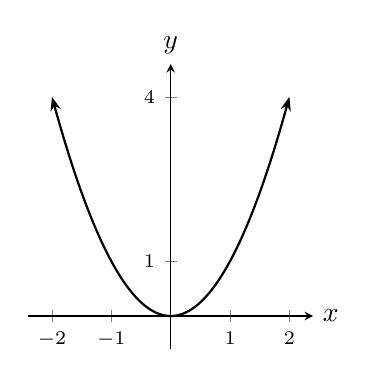
\begin{tikzpicture}
    \begin{axis}[
        width=5.2cm, height=5.2cm,
        axis lines=middle,
        xlabel={$x$}, ylabel={$y$},
        xmin=-2.4, xmax=2.4, ymin=-0.6, ymax=4.6,
        xtick={-2,-1,1,2}, ytick={1,4},
        tick label style={font=\scriptsize},
        every axis x label/.style={at={(ticklabel* cs:1)},anchor=west},
        every axis y label/.style={at={(ticklabel* cs:1)},anchor=south},
        clip=false
    ]
        \addplot[thick, domain=-2:2, samples=100, {Stealth[length=5pt]}-{Stealth[length=5pt]},] {x^2};

    \end{axis}
\end{tikzpicture}
\end{document}
